\chapter{进程管理与调度}

进程是操作系统选取某个可执行文件并对其进行一次动态执行的过程,它会对可执行文件提供硬件/虚拟资源,
同时在结束后也会进行资源的解绑。进程使得操作系统可以更动态灵活地管理和控制应用的执行。

\section{系统设计}

NimlothOS的进程管理系统采用三状态的进程模型,为每个用户程序提供独立的执行环境。
系统实现了基于时间片轮转(Round Robin)调度算法的抢占式多进程,并在后期实现了多级反馈队列(Multi-Level Feedback Queue, MLFQ)调度算法。
系统支持进程创建、切换、以及进程间通信。

进程管理系统的核心组件包括:

\begin{itemize}
    \item \textbf{进程控制块(ProcessControlBlock)}:存储进程的所有状态信息
    \item \textbf{进程管理器(ProcessManager)}:维护多级就绪队列,实现MLFQ调度策略
    \item \textbf{处理器抽象(Processor)}:管理当前运行进程,控制进程切换
    \item \textbf{PID分配器}:负责进程标识符的分配和回收
    \item \textbf{内核栈管理}:为每个进程分配独立的内核执行栈
    \item \textbf{信号系统}:实现进程间通信和控制机制
\end{itemize}

\section{进程状态转换}

进程在执行过程中会经历三种基本状态:

\begin{itemize}
    \item \textbf{就绪(Ready)}:进程已准备执行,等待分配CPU
    \item \textbf{运行(Running)}:进程正在CPU上执行
    \item \textbf{僵尸(Zombie)}:进程已结束,等待父进程回收
\end{itemize}

\section{调度策略}

一开始,我使用的是\textbf{时间片轮转(Round Robin)}调度策略,后来升级为更加先进的\textbf{多级反馈队列(Multi-Level Feedback Queue, MLFQ)}。

\section{时间片轮转调度}

时间片轮转调度是NimlothOS的第一个调度策略实现,它提供了一个简单的抢占式调度机制。

\subsection{时间片轮转调度算法}

时间片轮转调度算法是一种经典的抢占式调度策略,其核心思想是让所有进程公平地分享CPU资源。
系统控制流通过时钟中断实现强制进程切换,避免任何进程独占CPU,从而保证了调度的公平性——每个进程都能获得相等的CPU时间片。
这种时间片机制不仅确保系统能够快速响应用户交互,提供良好的响应性,同时算法实现相对简单,调度开销较低。
更重要的是,由于采用轮转的方式,所有就绪进程都能在有限时间内获得执行机会,有效避免了进程饥饿问题。

\subsection{时钟中断与抢占机制}

时间片轮转调度的核心在于时钟中断驱动的抢占机制。系统通过定期的时钟中断来强制进行进程切换,
确保没有进程能够无限期地占用CPU资源。它的实现涉及到硬件时钟、中断处理和进程调度三个模块的合作。

在NimlothOS中,时钟中断的处理流程如下:

\begin{lstlisting}[language=Rust,caption={时钟中断处理}, label={lst:timer-interrupt}]
// 在trap_handler中处理时钟中断
Trap::Interrupt(Interrupt::SupervisorTimer) => {
    next_trigger();                    // 设置下一次时钟中断
    suspend_current_and_run_next();    // 抢占当前进程并调度下一个
}
\end{lstlisting}

当时钟中断发生时,硬件会自动保存当前进程的基本状态(如PC和状态寄存器),
然后跳转到内核的中断处理程序。内核在处理完中断后,通过调用\lstinline[language=Rust]{suspend_current_and_run_next()}函数
将当前进程重新放入就绪队列的尾部,并从队列头部选择下一个进程执行,从而实现了公平的轮转调度。

RR调度算法下的进程调度全过程如下图所示。

\begin{figure}[htbp]
    \centering
    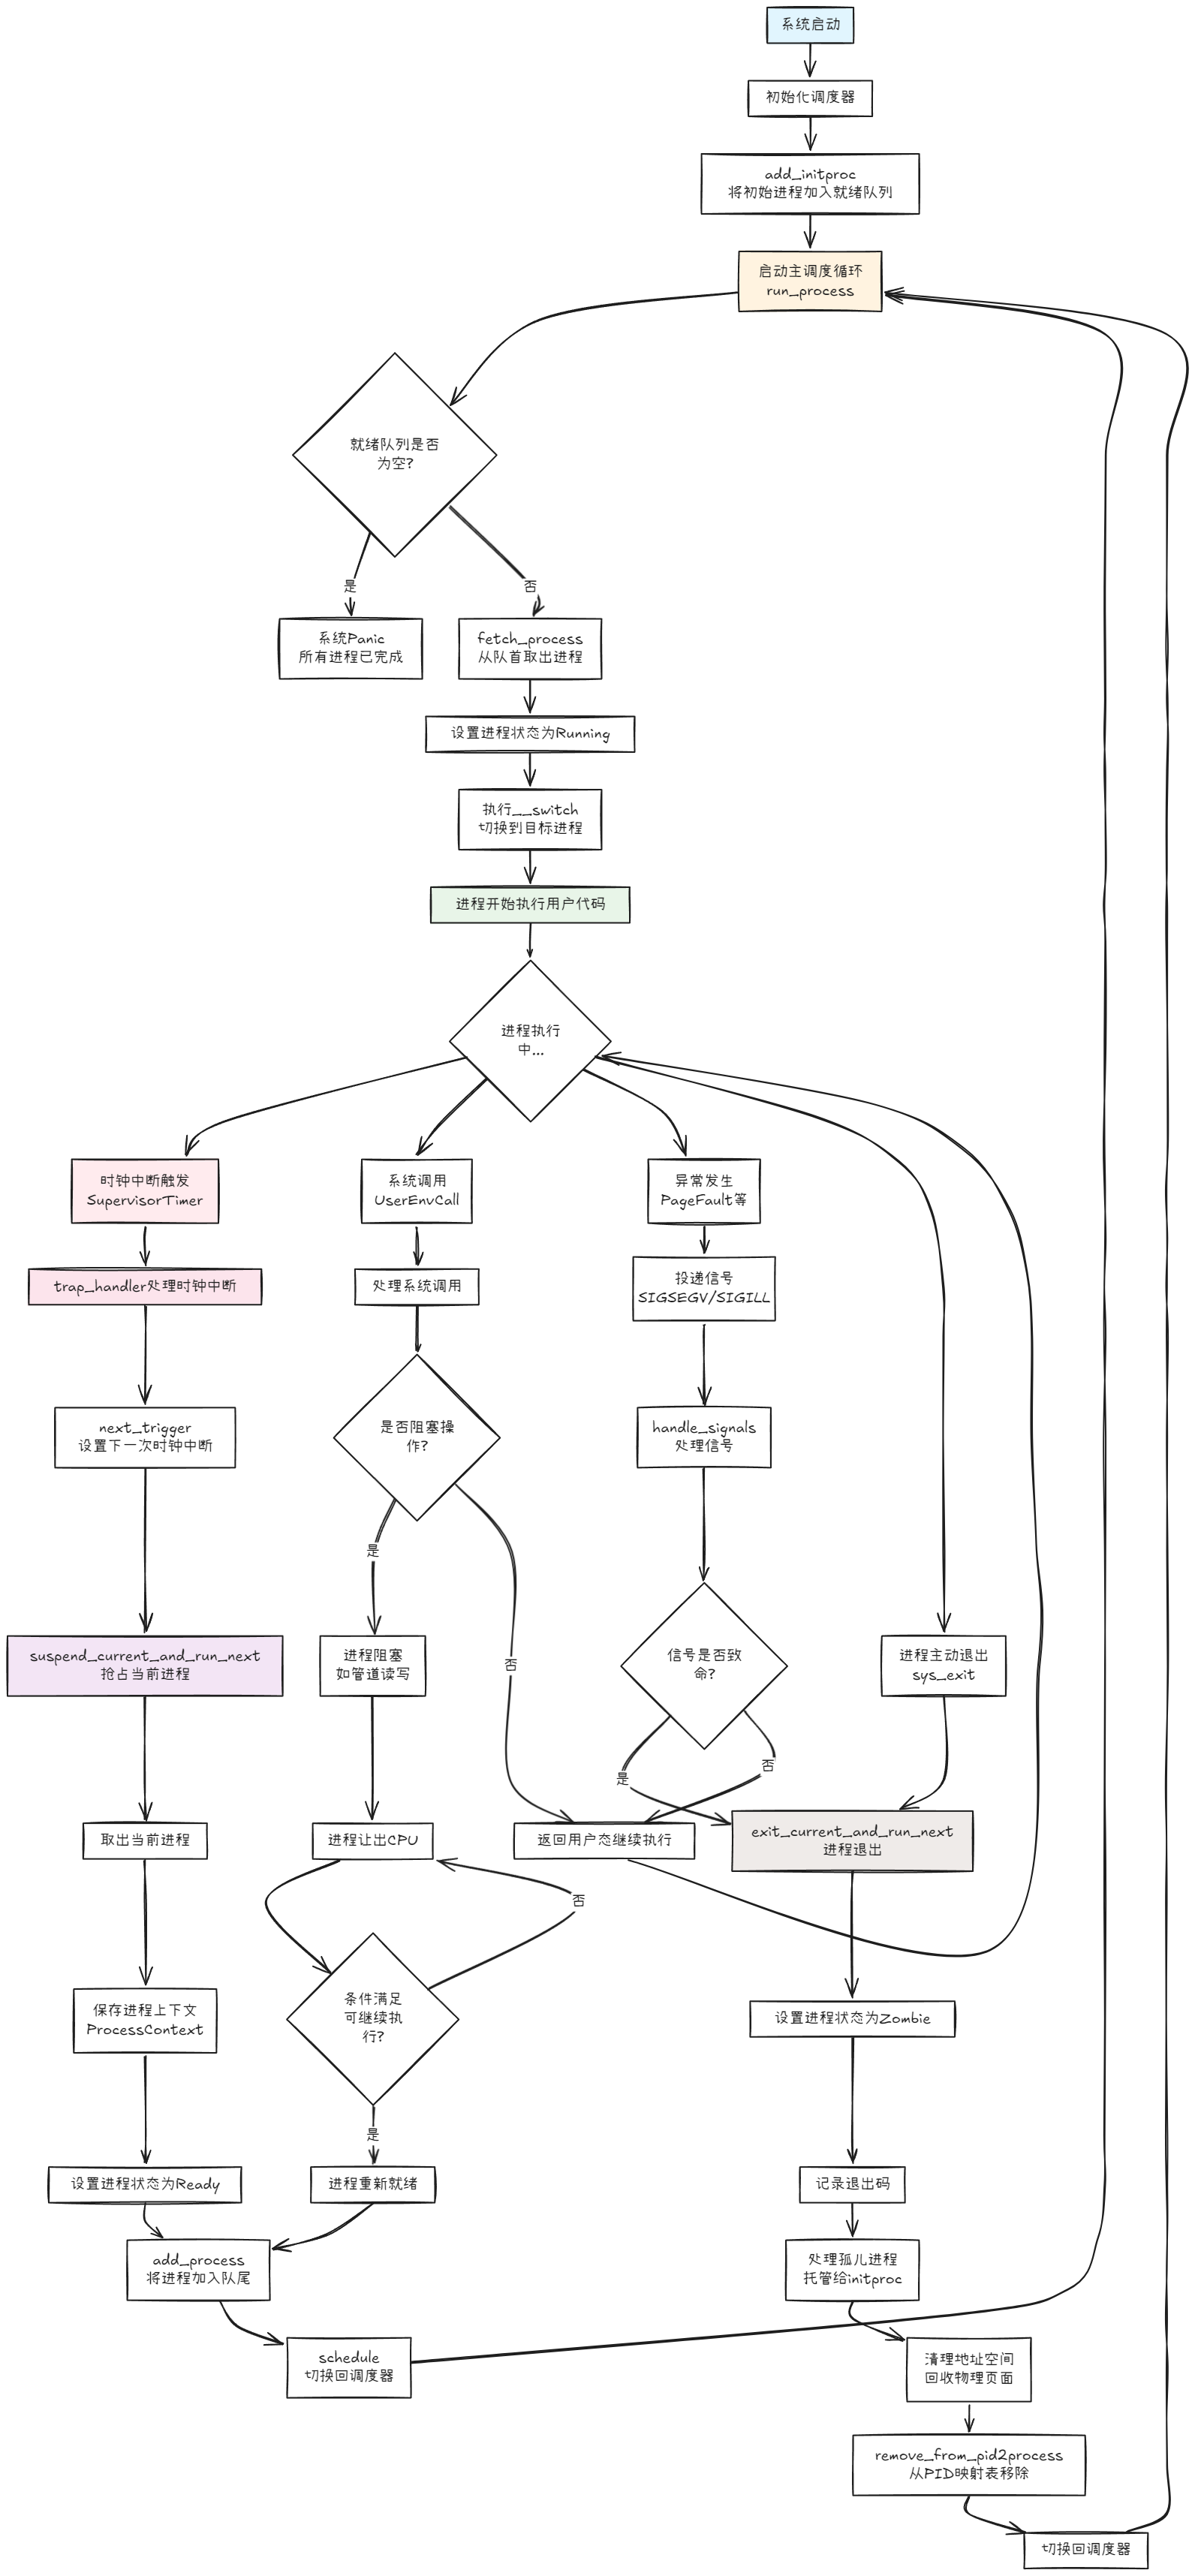
\includegraphics[width=0.7\textwidth]{../image/RR进程调度过程.png}
    \caption{RR调度算法下的进程调度全过程}
    \label{fig:rr-scheduling}
\end{figure}

\clearpage

\section{多级反馈队列调度}

为了克服时间片轮转调度在处理不同类型进程时的局限性,我将NimlothOS升级为了多级反馈队列(MLFQ)调度算法。
它结合了优先级调度和时间片轮转的优点,能够自适应地处理CPU密集型和I/O密集型进程,提供更好的系统响应性和吞吐量。
当然,它也有一定的缺陷,比如,CPU密集型进程的优先级下降很快,以及进程可以通过主动出让CPU来恶意欺骗系统调度器,
从而保持在更高的优先级。

\subsection{MLFQ调度算法}

多级反馈队列调度算法的核心思想是维护多个不同优先级的就绪队列,
并根据进程的行为特征动态调整其优先级。这种设计的智能之处在于它能够自适应地处理不同类型的工作负载。
系统维护多个优先级不同的就绪队列,调度时总是优先处理高优先级队列中的进程。
对于CPU密集型进程,算法会逐渐将其降级到低优先级队列,减少对交互性的影响;
而对于I/O密集型进程,系统会在其完成I/O操作后将其提升到高优先级队列,从而改善响应性。
通过为不同优先级队列配置不同长度的时间片,MLFQ在响应性和吞吐量之间实现了良好的平衡。
尽管采用了优先级机制,但算法仍能确保低优先级进程获得执行机会,有效防止了饥饿问题。

\subsection{队列结构与时间片设计}

NimlothOS的MLFQ实现使用4个优先级队列,时间片按指数增长:

\begin{lstlisting}[language=Rust,caption={MLFQ配置参数}, label={lst:mlfq-config}]
/// MLFQ 队列数量
pub const MLFQ_QUEUE_COUNT: usize = 4;
/// MLFQ 基础时间片 (时钟周期数)
pub const MLFQ_BASE_TIME_SLICE: usize = CLOCK_FREQ / 100; // 10ms
\end{lstlisting}

时间片分配策略如下:
\begin{itemize}
    \item \textbf{队列0(最高优先级)}:10ms - 适合交互式进程,快速响应
    \item \textbf{队列1}:20ms - 平衡响应性和效率
    \item \textbf{队列2}:40ms - 适合CPU密集型进程
    \item \textbf{队列3(最低优先级)}:80ms - 长时间片,提高吞吐量
\end{itemize}

这样,短作业和交互式进程可以获得更好的响应性,长时间运行的进程则获得更大的时间片以提高效率。

MLFQ调度算法下的进程调度全过程如下图所示。

\begin{figure}[htbp]
    \centering
    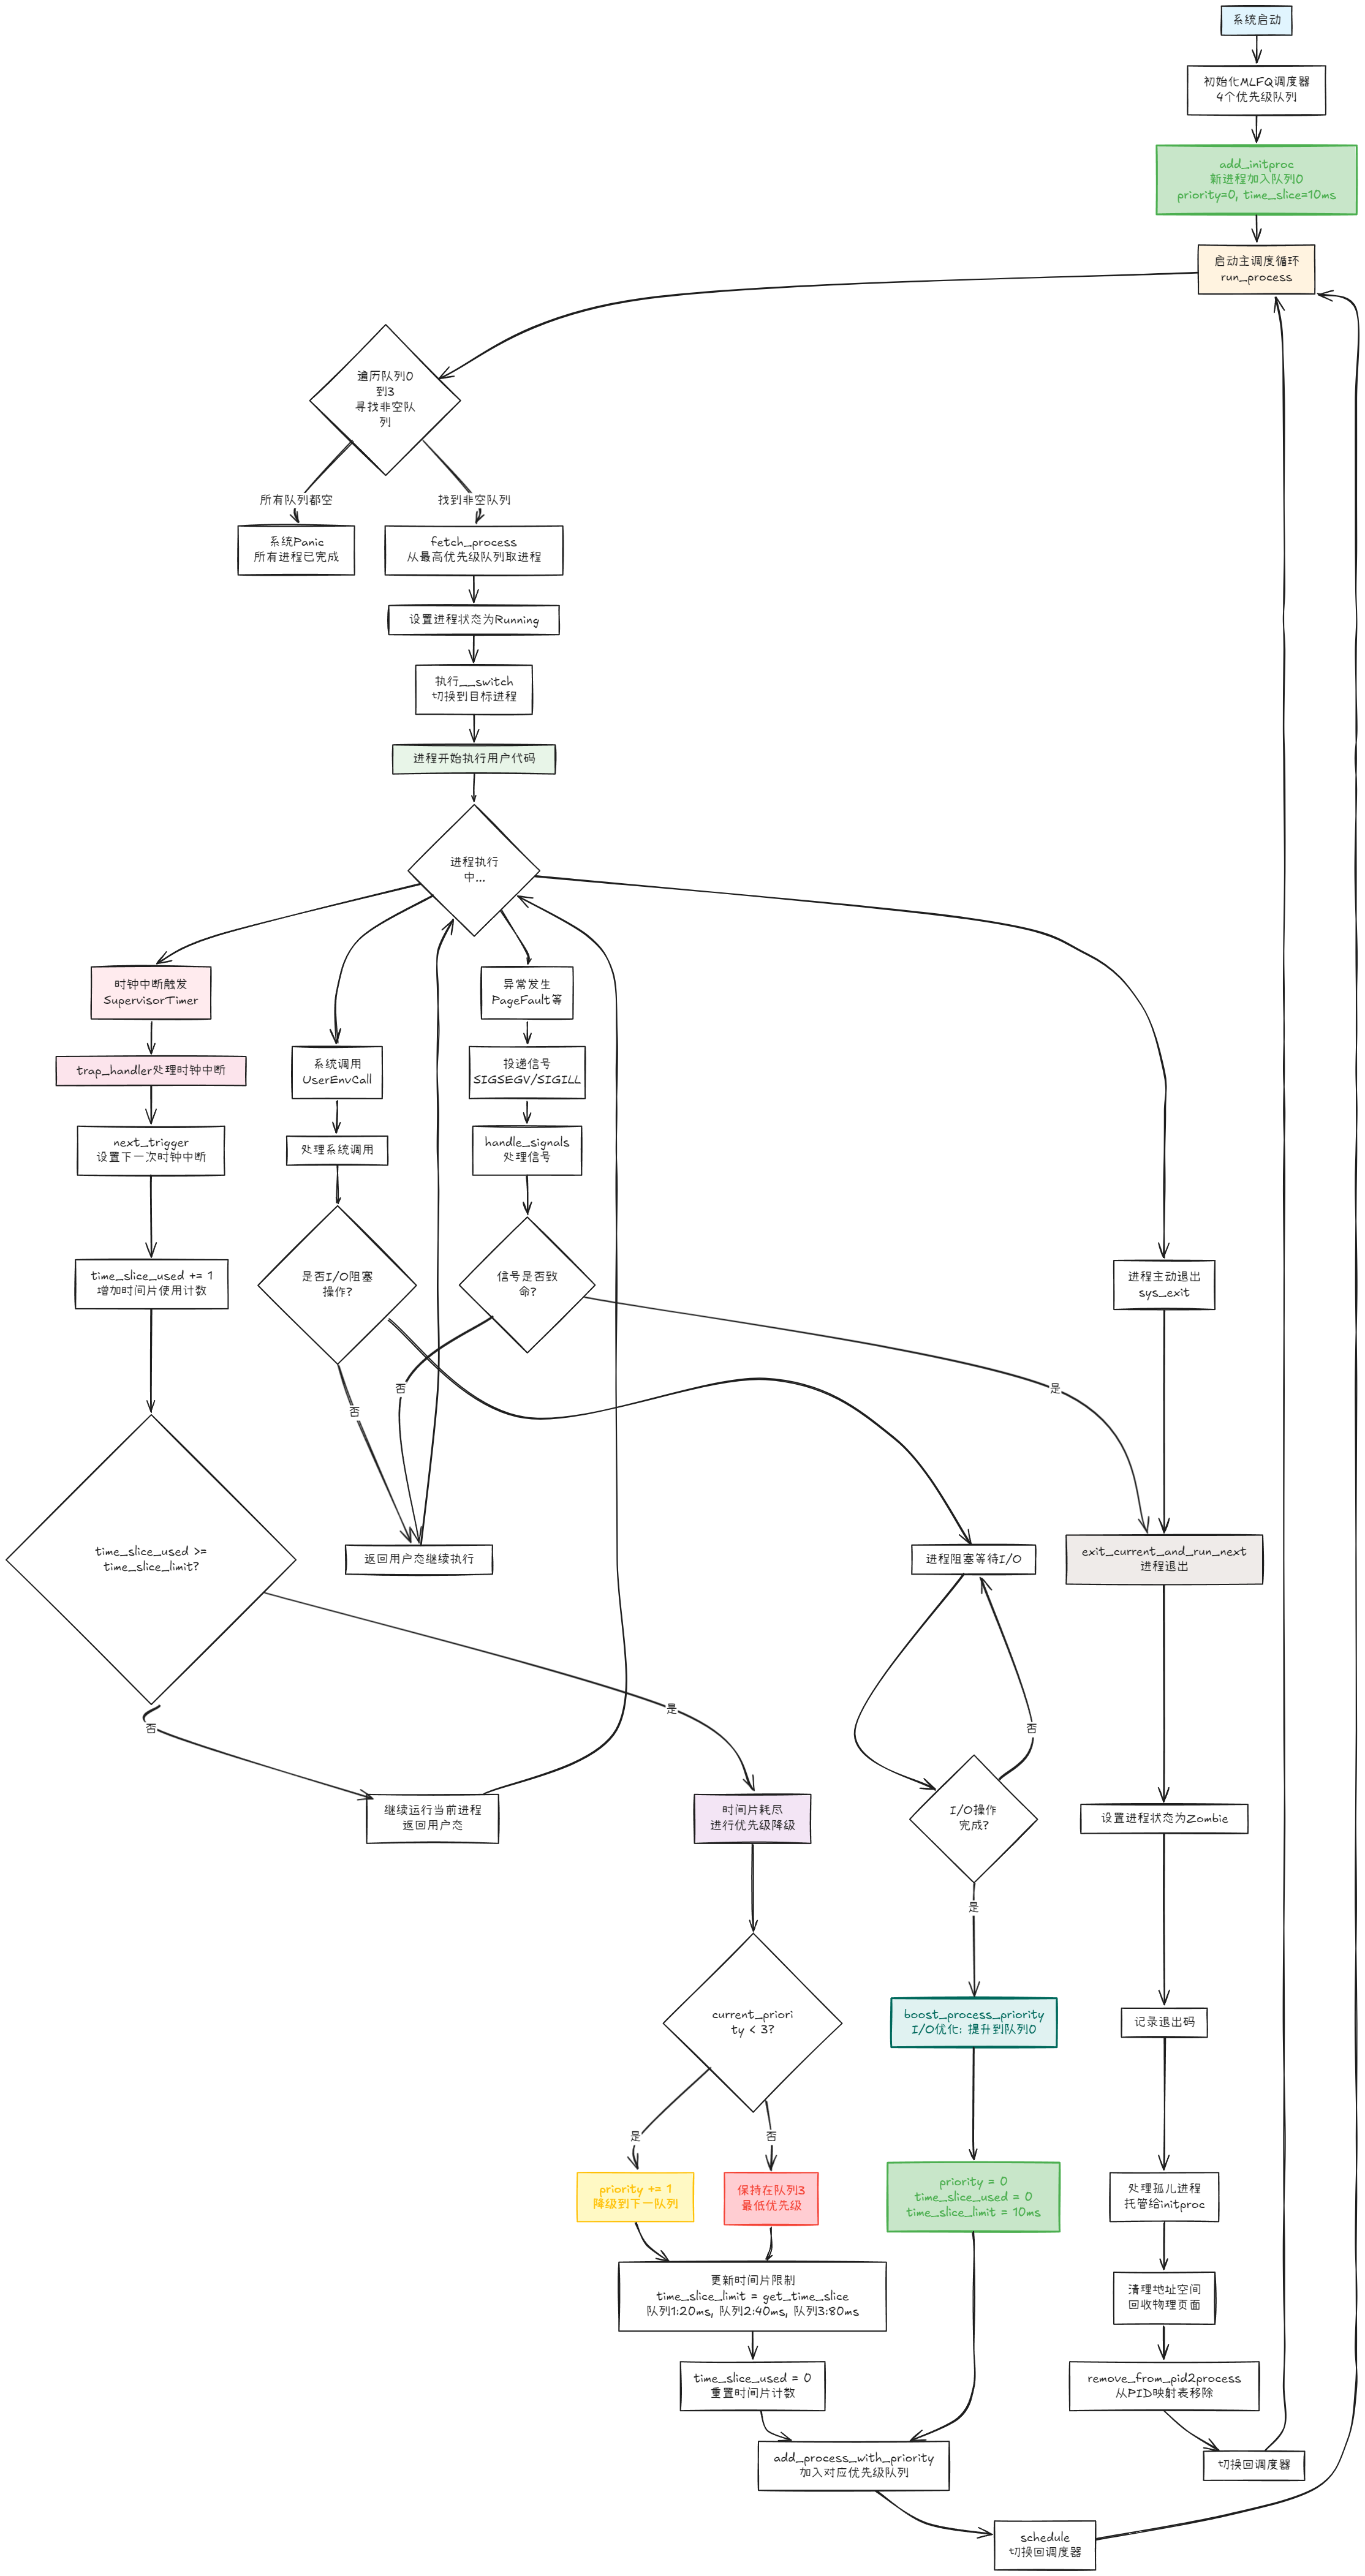
\includegraphics[width=0.8\textwidth]{../image/MLFQ进程调度过程.png}
    \caption{MLFQ调度算法下的进程调度全过程}
    \label{fig:mlfq-scheduling}
\end{figure}

\clearpage

\subsection{MLFQ数据结构实现}

多级反馈队列的实现基于向量化的队列结构,高优先级队列总是优先于低优先级队列被调度,
在队列内部,系统采用FIFO策略来维护公平性,确保同一优先级的进程得到公平对待。

\begin{lstlisting}[language=Rust,caption={MLFQ进程管理器结构}, label={lst:mlfq-manager}]
pub struct ProcessManager {
    /// 多级就绪进程队列
    ready_queues: Vec<VecDeque<Arc<ProcessControlBlock>>>,
    /// 每个队列的时间片长度(时钟周期数)
    time_slices: Vec<usize>,
    /// 队列数量
    queue_count: usize,
}

impl ProcessManager {
    pub fn new() -> Self {
        let mut ready_queues = Vec::new();
        let mut time_slices = Vec::new();
        // 初始化多级队列,时间片按优先级递增
        for i in 0..MLFQ_QUEUE_COUNT {
            ready_queues.push(VecDeque::new());
            // 时间片:10ms, 20ms, 40ms, 80ms
            time_slices.push(MLFQ_BASE_TIME_SLICE * (1 << i));
        }
        Self {
            ready_queues,
            time_slices,
            queue_count: MLFQ_QUEUE_COUNT,
        }
    }
}
\end{lstlisting}

\subsection{进程优先级与时间片管理}

每个进程在其控制块中维护MLFQ相关的状态信息:

\begin{lstlisting}[language=Rust,caption={进程MLFQ状态}, label={lst:process-mlfq-state}]
pub struct ProcessControlBlockInner {
    // ... 其他字段 ...
    /// MLFQ 调度优先级
    pub priority: usize,
    /// 当前时间片已使用的时钟周期数
    pub time_slice_used: usize,
    /// 当前优先级队列的时间片限制
    pub time_slice_limit: usize,
}
\end{lstlisting}

新创建的进程默认在最高优先级队列开始:

\begin{lstlisting}[language=Rust,caption={新进程优先级初始化}, label={lst:new-process-priority}]
// 新进程从最高优先级开始
priority: 0,
time_slice_used: 0,
time_slice_limit: MLFQ_BASE_TIME_SLICE,
\end{lstlisting}

这样可以确保新进程和短时间运行的进程获得最好的响应性。

\subsection{MLFQ调度策略实现}

MLFQ的调度决策遵循严格的优先级规则,同时在队列内部保持公平性:

\begin{lstlisting}[language=Rust,caption={MLFQ调度算法}, label={lst:mlfq-fetch}]
impl ProcessManager {
    /// 从最高优先级非空队列获取进程
    pub fn fetch(&mut self) -> Option<Arc<ProcessControlBlock>> {
        for queue in &mut self.ready_queues {
            if let Some(process) = queue.pop_front() {
                return Some(process);
            }
        }
        None
    }
    /// 向指定优先级队列添加进程
    pub fn add(&mut self, process: Arc<ProcessControlBlock>, priority: usize) {
        let queue_idx = priority.min(self.queue_count - 1);
        self.ready_queues[queue_idx].push_back(process);
    }
    /// 获取指定优先级队列的时间片长度
    pub fn get_time_slice(&self, priority: usize) -> usize {
        let queue_idx = priority.min(self.queue_count - 1);
        self.time_slices[queue_idx]
    }
}
\end{lstlisting}

\lstinline[language=Rust]{fetch()}函数通过遍历\lstinline[language=Rust]{ready_queues}向量来实现严格的优先级调度,
它从索引0(最高优先级)开始依次检查各个队列,一旦找到非空队列就立即取出进程,这保证了高优先级进程的优先执行。
\lstinline[language=Rust]{add()}方法负责将进程插入到指定优先级的队列尾部,通过\lstinline[language=Rust]{queue_idx.min(self.queue_count - 1)}确保优先级不会越界。
\lstinline[language=Rust]{get_time_slice()}方法根据优先级返回对应的时间片长度,实现了不同队列使用不同时间片的设计目标。

\subsection{优先级降级机制}

MLFQ的关键特性是根据进程行为动态调整其优先级。当进程用完其时间片时,
系统会将其降级到下一个优先级队列:

\begin{lstlisting}[language=Rust,caption={MLFQ时间片处理和降级}, label={lst:mlfq-downgrade}]
// 在trap_handler中处理时钟中断
Trap::Interrupt(Interrupt::SupervisorTimer) => {
    next_trigger();
    // MLFQ 时间片降级逻辑
    let process = current_process().unwrap();
    let mut inner = process.inner_exclusive_access();
    // 增加已使用时间片
    inner.time_slice_used += 1;
    if inner.time_slice_used >= inner.time_slice_limit {
        // 时间片耗尽,进行降级
        let current_priority = inner.priority;
        let new_priority = if current_priority < MLFQ_QUEUE_COUNT - 1 {
            current_priority + 1  // 降级到下一队列
        } else {
            current_priority      // 已在最低优先级
        };
        // 更新进程优先级和时间片
        inner.priority = new_priority;
        inner.time_slice_used = 0;
        inner.time_slice_limit = get_time_slice(new_priority);
        drop(inner);
        // 重新入队到对应优先级队列
        add_process_with_priority(process, new_priority);
        // 切换到调度器
        schedule(process_cx_ptr);
    } else {
        // 时间片未耗尽,继续运行当前进程
        drop(inner);
    }
}
\end{lstlisting}

\subsection{I/O优化与优先级提升}

MLFQ的另一个特性是对I/O密集型进程的优化。当进程完成I/O操作后,
系统会恢复甚至提升其优先级,以改善交互响应性:

这个机制暂时还没使用。它应该在进程从I/O等待中恢复、或者从子进程等待中恢复、
或是从sleep中唤醒时被调用。另外后续还需要完善防饥饿机制,
比如检查是否有进程在低级别队列停留过久。

\subsection{MLFQ vs RR 对比}

\begin{table}[htbp]
\centering
\caption{MLFQ与RR调度策略对比}
\label{tab:mlfq-vs-rr}
\begin{tabular}{|l|l|l|}
\hline
\textbf{特性} & \textbf{Round Robin} & \textbf{MLFQ} \\
\hline
响应时间 & 固定时间片 & 短作业快速响应 \\
\hline
吞吐量 & 频繁切换,吞吐量中等 & 长作业大时间片,吞吐量高 \\
\hline
公平性 & 绝对公平 & 相对公平,偏向短作业 \\
\hline
交互性 & 所有进程同等对待 & 自动识别交互式进程 \\
\hline
\end{tabular}
\end{table}

\noindent
\rule{0.4\textwidth}{0.4pt}
\hfill
\text{以下为实现介绍}
\hfill
\rule{0.4\textwidth}{0.4pt}

\section{进程上下文管理}

进程上下文是进程切换机制的核心,它保存了进程在被暂停时的完整CPU状态,
使得进程可以在稍后恢复到完全相同的执行状态。

\subsection{进程上下文结构}

进程上下文的定义如下:

\begin{lstlisting}[language=Rust,caption={进程上下文结构}, label={lst:process-context}]
#[repr(C)]
#[derive(Copy, Clone)]
pub struct ProcessContext {
    /// 返回地址寄存器 (ra)
    ra: usize,
    /// 栈指针寄存器 (sp)
    sp: usize,
    /// 被调用者保存寄存器 (s0-s11)
    s: [usize; 12],
}
\end{lstlisting}

这个结构体的字段设计遵循RISC-V调用约定。\lstinline[language=Rust]{ra}字段保存返回地址寄存器,
进程恢复时CPU会跳转到此地址继续执行。\lstinline[language=Rust]{sp}字段存储栈指针,指向进程的内核栈顶位置。
\lstinline[language=Rust]{s: [usize; 12]}数组保存s0到s11这12个被调用者保存寄存器,
这些寄存器在函数调用过程中必须保持值不变,因此在进程切换时需要明确保存和恢复。
整个结构体总共保存14个寄存器状态,这是RISC-V架构下实现进程上下文切换的最小必要集合。

\subsection{上下文创建与初始化}

系统提供两种创建进程上下文的方式:

\begin{lstlisting}[language=Rust,caption={上下文创建方法}, label={lst:context-creation}]
impl ProcessContext {
    /// 创建零初始化的进程上下文
    pub fn zero_init() -> Self {
        Self {
            ra: 0,
            sp: 0,
            s: [0; 12],
        }
    }
    /// 创建指向陷阱返回的进程上下文
    pub fn goto_trap_return(kstack_ptr: usize) -> Self {
        Self {
            ra: trap_return as usize,
            sp: kstack_ptr,
            s: [0; 12],
        }
    }
}
\end{lstlisting}

\lstinline[language=Rust]{goto_trap_return}方法为新进程创建特殊的启动上下文,
使得进程首次被调度时能够通过\lstinline[language=Rust]{trap_return}函数正确进入用户态。

\section{进程控制块}

进程控制块(ProcessControlBlock, PCB)是进程的核心数据结构,包含了进程运行所需的所有信息。

\subsection{PCB结构设计}

\begin{lstlisting}[language=Rust,caption={进程控制块结构}, label={lst:pcb-structure}]
pub struct ProcessControlBlock {
    /// 进程标识符句柄
    pub pid: PidHandle,
    /// 内核栈
    pub kernel_stack: KernelStack,
    /// 内部可变状态
    inner: UPSafeCell<ProcessControlBlockInner>,
}
pub struct ProcessControlBlockInner {
    /// 进程当前状态
    pub process_status: ProcessStatus,
    /// 进程上下文
    pub process_cx: ProcessContext,
    /// 进程地址空间
    pub memory_set: MemorySet,
    /// 陷阱上下文物理页号
    pub trap_cx_ppn: PhysPageNum,
    /// 进程基础内存大小
    pub base_size: usize,
    /// 父进程引用
    pub parent: Option<Weak<ProcessControlBlock>>,
    /// 子进程列表
    pub children: Vec<Arc<ProcessControlBlock>>,
    /// 进程退出码
    pub exit_code: i32,
    /// 文件描述符表
    pub fd_table: Vec<Option<Arc<dyn File + Send + Sync>>>,
    // 信号相关字段
    pub signals: SignalFlags,
    pub signal_mask: SignalFlags,
    pub handling_sig: isize,
    pub signal_actions: SignalActions,
    pub killed: bool,
    pub frozen: bool,
    pub trap_ctx_backup: Option<TrapContext>,
    /// MLFQ 调度优先级
    pub priority: usize,
    /// 当前时间片已使用的时钟周期数
    pub time_slice_used: usize,
    /// 当前优先级队列的时间片限制
    pub time_slice_limit: usize,
}
\end{lstlisting}

PCB的设计采用了分层结构,这样可以分离当中的不变数据和可变数据,并加以保护。

\begin{itemize}
    \item \textbf{外层结构}:包含不变的基础信息,如PID和内核栈。这些资源在进程生命周期中保持不变,
    可以安全地在多个调度器组件间共享,无需额外的同步保护。
    \item \textbf{内层结构}:包含运行时可变的状态信息,通过\lstinline[language=Rust]{UPSafeCell}保护。
    这样可以使进程状态的修改操作具有原子性,避免在进程切换过程中出现竞态条件。
\end{itemize}

这样设计的原因在于:首先,它最小化了需要同步保护的数据范围,提高了系统性能;
其次,将不变数据与可变数据分离,使得代码更加清晰和安全;最后,通过RAII机制,
外层资源(如PID和内核栈)的生命周期与PCB严格绑定,避免了资源泄漏问题。

\subsection{进程创建}

新进程的创建是操作系统中最复杂的操作之一,需要协调多个子系统来建立完整的进程执行环境。
NimlothOS的进程创建使用"加载-初始化-激活"的三阶段模式,确保新进程能够在正确的隔离环境中开始执行。

整个创建过程可以分解为以下步骤:
\begin{enumerate}
    \item \textbf{ELF解析阶段}:解析可执行文件格式,提取程序段信息和入口点
    \item \textbf{地址空间建立}:创建进程专用的虚拟地址空间和页表
    \item \textbf{资源分配}:分配PID、内核栈等系统资源
    \item \textbf{上下文初始化}:设置进程的初始执行状态
    \item \textbf{环境准备}:初始化文件描述符表、信号处理等运行环境
\end{enumerate}

这样确保了进程在创建完成时就拥有了完整的执行环境,可以立即被调度器选中执行。
下面的代码展示了这个过程的具体实现:

\begin{lstlisting}[language=Rust,caption={进程创建过程}, label={lst:process-creation}]
impl ProcessControlBlock {
    pub fn new(elf_data: &[u8]) -> Self {
        // 解析ELF文件并创建地址空间
        let (memory_set, user_sp, entry_point) = MemorySet::from_elf(elf_data);
        let trap_cx_ppn = memory_set
            .translate(VirtAddr::from(TRAP_CONTEXT).into())
            .unwrap()
            .ppn();
        // 分配PID和内核栈
        let pid_handle = pid_alloc();
        let kernel_stack = KernelStack::new(&pid_handle);
        let kernel_stack_top = kernel_stack.top();
        // 创建进程控制块
        let process_control_block = Self {
            pid: pid_handle,
            kernel_stack,
            inner: unsafe {
                UPSafeCell::new(ProcessControlBlockInner {
                    process_status: ProcessStatus::Ready,
                    process_cx: ProcessContext::goto_trap_return(kernel_stack_top),
                    memory_set,
                    trap_cx_ppn,
                    base_size: user_sp,
                    parent: None,
                    children: Vec::new(),
                    exit_code: 0,
                    fd_table: vec![
                        Some(Arc::new(Stdin)),
                        Some(Arc::new(Stdout)),
                        Some(Arc::new(Stderr)),
                    ],
                    signals: SignalFlags::empty(),
                    signal_mask: SignalFlags::empty(),
                    handling_sig: -1,
                    signal_actions: SignalActions::default(),
                    killed: false,
                    frozen: false,
                    trap_ctx_backup: None,
                    priority: 0, // 新进程从最高优先级开始
                    time_slice_used: 0,
                    time_slice_limit: {
                        use crate::config::MLFQ_BASE_TIME_SLICE;
                        MLFQ_BASE_TIME_SLICE
                    },
                })
            },
        };
        // 初始化陷阱上下文
        let trap_ctx = process.inner_exclusive_access().trap_cx();
        *trap_ctx = TrapContext::app_init_context(
            entry_point,
            user_sp,
            KERNEL_SPACE.exclusive_access().token(),
            kernel_stack_top,
            trap_handler as usize,
        );
        process_control_block
    }
}
\end{lstlisting}

\section{进程管理器}

进程管理器负责维护多级就绪队列,配合时钟中断实现多级反馈队列(MLFQ)调度策略。

\subsection{管理器结构}

\begin{lstlisting}[language=Rust,caption={MLFQ进程管理器结构}, label={lst:mlfq-process-manager}]
pub struct ProcessManager {
    /// 多级就绪进程队列
    ready_queues: Vec<VecDeque<Arc<ProcessControlBlock>>>,
    /// 每个队列的时间片长度(时钟周期数)
    time_slices: Vec<usize>,
    /// 队列数量
    queue_count: usize,
}

impl ProcessManager {
    /// 向指定优先级队列添加进程
    pub fn add(&mut self, process: Arc<ProcessControlBlock>, priority: usize) {
        let queue_idx = priority.min(self.queue_count - 1);
        self.ready_queues[queue_idx].push_back(process);
    }

    /// 从最高优先级非空队列获取进程
    pub fn fetch(&mut self) -> Option<Arc<ProcessControlBlock>> {
        for queue in &mut self.ready_queues {
            if let Some(process) = queue.pop_front() {
                return Some(process);
            }
        }
        None
    }

    /// 获取指定优先级队列的时间片长度
    pub fn get_time_slice(&self, priority: usize) -> usize {
        let queue_idx = priority.min(self.queue_count - 1);
        self.time_slices[queue_idx]
    }
}
\end{lstlisting}

MLFQ进程管理器使用\lstinline[language=Rust]{Vec<VecDeque>}构建多级队列结构。
\lstinline[language=Rust]{add()}方法根据优先级参数将进程插入到对应的队列中,通过\lstinline[language=Rust]{queue_idx.min(self.queue_count - 1)}确保索引不越界。
\lstinline[language=Rust]{fetch()}方法体现了MLFQ的核心调度逻辑:从索引0开始遍历各个优先级队列,
一旦找到非空队列就立即取出进程,这保证了高优先级进程总是优先被调度。
\lstinline[language=Rust]{get_time_slice()}方法为不同优先级队列提供不同的时间片长度,实现MLFQ的差异化调度策略。

\subsection{全局管理器实例}

\lstinline[language=Rust]{PROCESS_MANAGER}维护多级就绪队列用于调度决策,
而\lstinline[language=Rust]{PID2PCB}作为\lstinline[language=Rust]{BTreeMap}提供从PID到进程控制块的快速映射。
系统提供两个进程添加接口:\lstinline[language=Rust]{add_process()}将新进程默认加入最高优先级队列(priority=0),
而\lstinline[language=Rust]{add_process_with_priority()}允许指定具体的优先级队列。
两个函数都会同步更新PID映射表和MLFQ队列,确保数据结构的一致性。

\begin{lstlisting}[language=Rust,caption={全局进程管理器}, label={lst:global-manager}]
lazy_static! {
    /// 全局进程管理器实例
    pub static ref PROCESS_MANAGER: UPSafeCell<ProcessManager> =
        unsafe { UPSafeCell::new(ProcessManager::new()) };
    /// PID到进程控制块的映射
    pub static ref PID2PCB: UPSafeCell<BTreeMap<usize, Arc<ProcessControlBlock>>> =
        unsafe { UPSafeCell::new(BTreeMap::new()) };
}

/// 向全局MLFQ队列添加进程(默认最高优先级)
pub fn add_process(process: Arc<ProcessControlBlock>) {
    PID2PCB
        .exclusive_access()
        .insert(process.getpid(), Arc::clone(&process));
    PROCESS_MANAGER.exclusive_access().add(process, 0);
}

/// 向指定优先级队列添加进程
pub fn add_process_with_priority(process: Arc<ProcessControlBlock>, priority: usize) {
    PID2PCB
        .exclusive_access()
        .insert(process.getpid(), Arc::clone(&process));
    PROCESS_MANAGER.exclusive_access().add(process, priority);
}

/// 从全局进程管理器获取下一个待调度进程
pub fn fetch_process() -> Option<Arc<ProcessControlBlock>> {
    PROCESS_MANAGER.exclusive_access().fetch()
}
\end{lstlisting}

\section{处理器抽象}

处理器抽象管理当前运行的进程,并控制进程切换操作。可以分为系统控制流抽象和普通进程的抽象。它们会在进程切换时进行切换,
并由系统控制流来完成切换到下一个进程Processor抽象的操作。

\subsection{处理器结构}

\begin{lstlisting}[language=Rust,caption={处理器抽象结构}, label={lst:processor-structure}]
pub struct Processor {
    /// 当前正在执行的进程
    current: Option<Arc<ProcessControlBlock>>,
    /// 空闲进程上下文(调取器)
    idle_process_cx: ProcessContext,
}
\end{lstlisting}

\subsection{主调度循环}

调度器的核心是\lstinline[language=Rust]{run_process}函数实现的主调度循环。这个函数体现了操作系统的核心工作模式:
持续不断地为系统中的进程分配CPU时间,确保所有进程都能得到执行机会。

主调度循环采用了"无限循环+事件驱动"的设计模式,它会永不停歇地运行在系统的idle控制流中,也即主调度进程中,
负责在进程间进行上下文切换。它本身并不运行任何用户代码,而是作为一个调度器,决定哪个进程应该获得CPU控制权。

调度决策基于MLFQ策略:总是选择最高优先级非空队列中的进程执行,每个进程根据其优先级队列
分配不同长度的时间片,时间片耗尽后进程可能被降级到低优先级队列。这种策略通过动态优先级调整
实现了对不同类型工作负载的自适应优化,既保证了交互式进程的响应性,又提高了CPU密集型进程的吞吐量。当没有进程可调度时,系统会进入panic状态,
这表明所有应用程序都已完成执行。

下面的实现展示了这个关键组件的工作机制:

\begin{lstlisting}[language=Rust,caption={主调度循环}, label={lst:main-scheduler}]
pub fn run_process() {
    loop {
        let mut processor = PROCESSOR.exclusive_access();
        if let Some(process) = fetch_process() {
            let idle_process_cx_ptr = processor.idle_process_cx_ptr();
            // 获取进程上下文指针
            let mut process_inner = process.inner_exclusive_access();
            let next_process_cx_ptr = &process_inner.process_cx as *const ProcessContext;
            process_inner.process_status = ProcessStatus::Running;
            drop(process_inner);
            
            // 设置当前进程
            processor.current = Some(process);
            drop(processor);
            
            // 执行进程切换
            unsafe {
                __switch(idle_process_cx_ptr, next_process_cx_ptr);
            }
        } else {
            panic!("no processes available in run_process");
        }
    }
}
\end{lstlisting}

调度循环的工作流程:
\begin{enumerate}
    \item 从就绪队列获取下一个进程
    \item 将进程状态设置为Running
    \item 执行底层上下文切换
    \item 进程运行直到主动让出CPU或被抢占
    \item 回到调度循环,选择下一个进程
\end{enumerate}

\subsection{进程切换}

回到主循环调度进程的进程切换通过\lstinline[language=Rust]{schedule}函数实现:

\begin{lstlisting}[language=Rust,caption={进程切换实现}, label={lst:process-switch}]
pub fn schedule(switched_process_cx_ptr: *mut ProcessContext) {
    let mut processor = PROCESSOR.exclusive_access();
    let idle_process_cx_ptr = processor.idle_process_cx_ptr();
    drop(processor);
    unsafe {
        __switch(switched_process_cx_ptr, idle_process_cx_ptr);
    }
}
\end{lstlisting}

\section{底层切换机制}

进程切换的底层实现由汇编代码\lstinline[language=Rust]{__switch}完成,这是整个进程管理系统中最关键的底层机制。
它直接操作CPU寄存器,实现进程间的原子级切换。

\lstinline[language=Rust]{__switch}函数设计遵循RISC-V调用约定,它接受两个参数:当前进程的上下文指针(a0寄存器)
和目标进程的上下文指针(a1寄存器)。这样使得切换操作对调用者而言是透明的——
函数返回时,执行环境已经切换到了目标进程,但调用语义保持不变。

切换过程的原子性很关键:在保存完当前进程状态之前,不能被中断打断;
在恢复目标进程状态的过程中,也必须保持原子性。这通过中断处理程序进行保护,
\lstinline[language=Rust]{trap_handler}函数会保存所有相关的寄存器。

汇编使用RISC-V的宏机制来处理重复性的寄存器操作。

\begin{lstlisting}[language={[x86masm]Assembler},caption={底层上下文切换}, label={lst:low-level-switch}]
.altmacro
.macro SAVE_SN n
    sd s\n, (\n+2)*8(a0)
.endm
.macro LOAD_SN n
    ld s\n, (\n+2)*8(a1)
.endm

    .section .text
    .globl __switch
__switch:
    # 保存当前进程上下文到a0指向的内存
    sd ra, 0*8(a0)
    sd sp, 1*8(a0)
    .set n, 0
    .rept 12
        SAVE_SN %n
        .set n, n + 1
    .endr

    # 从a1指向的内存恢复目标进程上下文
    ld ra, 0*8(a1)
    ld sp, 1*8(a1)
    .set n, 0
    .rept 12
        LOAD_SN %n
        .set n, n + 1
    .endr

    ret
\end{lstlisting}

切换过程包含两个阶段:

\begin{enumerate}
    \item \textbf{保存阶段}:将当前进程的寄存器状态保存到其ProcessContext中。首先保存返回地址(ra)
    和栈指针(sp),然后依次保存所有被调用者保存寄存器(s0-s11)。保存操作使用偏移量计算来定位
    ProcessContext结构体中的相应字段,确保数据的正确存储。
    
    \item \textbf{恢复阶段}:从目标进程的ProcessContext中恢复寄存器状态。恢复的顺序与保存相同:
    先恢复ra和sp,再恢复s0-s11。恢复完成后,通过\lstinline[language={[x86masm]Assembler}]{ret}指令
    跳转到目标进程的返回地址,完成整个切换过程。
\end{enumerate}

这样设计使得\lstinline[language=Rust]{__switch}函数"返回"时,就已经在目标进程的上下文中执行了。
调用者无需了解底层的切换细节,只需要按照普通函数调用的方式使用即可。

\section{PID与内核栈管理}

另外,之前提到在进程PCB中除了PCB\_Inner是可变的,还有两个不变的部分,即进程的PID和进程的内核栈。
系统实现了PID分配器和内核栈管理机制,为每个进程提供唯一标识和独立的内核执行环境。

\subsection{PID分配器}

\begin{lstlisting}[language=Rust,caption={PID分配器实现}, label={lst:pid-allocator}]
pub struct PidAllocator {
    /// 下一个要分配的新PID
    current: usize,
    /// 回收的PID池
    recycled: Vec<usize>,
}

impl PidAllocator {
    /// 分配新的PID
    pub fn alloc(&mut self) -> PidHandle {
        if let Some(pid) = self.recycled.pop() {
            PidHandle(pid)
        } else {
            self.current += 1;
            PidHandle(self.current - 1)
        }
    }
    /// 回收PID
    pub fn dealloc(&mut self, pid: usize) {
        assert!(pid < self.current);
        assert!(
            !self.recycled.iter().any(|ppid| *ppid == pid),
            "pid {} has been deallocated!",
            pid
        );
        self.recycled.push(pid);
    }
}
\end{lstlisting}

PID分配策略:
\begin{itemize}
    \item 优先复用回收池中的PID
    \item 回收池为空时分配新的递增PID
    \item 通过RAII机制自动管理PID生命周期
\end{itemize}

\subsection{内核栈管理}

每个进程都拥有独立的内核栈,用于系统调用和中断处理:

\begin{lstlisting}[language=Rust,caption={内核栈实现}, label={lst:kernel-stack}]
pub struct KernelStack {
    pid: usize,
}

impl KernelStack {
    /// 为指定进程创建内核栈
    pub fn new(pid_handle: &PidHandle) -> Self {
        let pid = pid_handle.0;
        let (kernel_stack_bottom, kernel_stack_top) = kernel_stack_position(pid);
        KERNEL_SPACE.exclusive_access().insert_framed_area(
            kernel_stack_bottom.into(),
            kernel_stack_top.into(),
            MapPermission::R | MapPermission::W,
        );
        KernelStack { pid: pid_handle.0 }
    }

    /// 获取内核栈顶地址
    pub fn top(&self) -> usize {
        let (_, kernel_stack_top) = kernel_stack_position(self.pid);
        kernel_stack_top
    }
}

/// 计算内核栈虚拟地址位置
pub fn kernel_stack_position(app_id: usize) -> (usize, usize) {
    let top = TRAMPOLINE - (KERNEL_STACK_SIZE + PAGE_SIZE) * app_id;
    let bottom = top - KERNEL_STACK_SIZE;
    (bottom, top)
}
\end{lstlisting}

内核栈固定大小为8KB,上一章也提到了,内核栈在内核地址空间中位于高地址的256GB,从TRAMPOLINE页往下
扩展,两个内核栈间还有一个保护页。它们通过唯一PID来标识。

\section{进程间通信机制}

NimlothOS实现了多种进程间通信(IPC)机制,为进程提供了数据交换、同步控制和协调工作的能力。
主要包括信号系统、管道通信和文件描述符继承机制。

\subsection{信号系统}

信号系统是NimlothOS中最基础的进程间通信机制,它是一种异步通信方式,
使得进程能够响应系统事件、错误条件和其他进程的控制请求。与传统的同步通信机制不同,
信号采用"发送即忘记"的语义,发送方无需等待接收方的响应,这使得信号特别适合用于
事件通知、错误报告和进程控制等场景。

NimlothOS的信号系统设计借鉴了POSIX标准,但进行了适当的简化以适应微内核架构的需求。
系统支持标准信号集合,包括致命信号(如SIGSEGV、SIGKILL)、控制信号(如SIGSTOP、SIGCONT)
和用户定义信号。每个信号都有明确的语义和默认处理行为,同时支持用户程序自定义处理逻辑。

信号处理的异步特性是其核心特征:信号可以在进程执行的任何时刻到达,进程必须能够
在适当的时机检查和处理这些信号。这种异步性既提供了灵活性,也带来了复杂性——
系统必须确保信号处理不会破坏进程的正常执行流程。

\subsubsection{信号标志与动作}

\begin{lstlisting}[language=Rust,caption={信号标志定义}, label={lst:signal-flags}]
bitflags! {
    pub struct SignalFlags: i32 {
        const SIGINT    = 1 << 2;  // 中断信号
        const SIGILL    = 1 << 4;  // 非法指令
        const SIGABRT   = 1 << 6;  // 异常终止
        const SIGFPE    = 1 << 8;  // 浮点异常
        const SIGKILL   = 1 << 9;  // 终止信号(不可捕捉)
        const SIGSEGV   = 1 << 11; // 内存访问错误
        const SIGPIPE   = 1 << 13; // 管道错误
        const SIGALRM   = 1 << 14; // 定时器信号
        const SIGTERM   = 1 << 15; // 终止请求
        const SIGSTOP   = 1 << 19; // 停止执行(不可捕捉)
        const SIGCONT   = 1 << 18; // 继续执行
        const SIGDEF    = 1 << 31; // 默认信号
    }
}

pub struct SignalAction {
    pub handler: usize,     // 处理程序地址
    pub mask: SignalFlags,  // 处理期间屏蔽的信号
}
\end{lstlisting}

系统支持标准的POSIX信号,每个信号都有特定的语义和默认处理方式。信号标志使用位域(bitflags)实现,
这种设计允许高效的信号集合操作,如信号合并、屏蔽和检查。\lstinline[language=Rust]{SignalAction}结构
定义了信号的处理方式,包括处理程序地址和在处理期间需要屏蔽的其他信号,这样可以防止信号处理过程中的重入问题。

\subsubsection{信号处理流程}

信号处理是一个多阶段的复杂过程,涉及信号投递、检查、屏蔽和处理等多个环节。
NimlothOS采用了"延迟处理"策略:信号在投递时并不立即处理,而是在进程的安全点
(如系统调用返回、时间片切换等)进行批量处理。这种设计避免了在任意执行点处理信号
可能带来的竞态条件和状态不一致问题。

信号处理的核心在于如何在保证进程正常执行的同时,及时响应异步事件。
系统采用了循环检查的方式,持续扫描进程的待决信号集合,并根据信号类型和当前进程状态
决定相应的处理动作。对于冻结状态的进程,系统会自动让出CPU,等待解冻信号的到达。

\begin{lstlisting}[language=Rust,caption={信号处理实现}, label={lst:signal-handling}]
/// 处理当前进程的待决信号
pub fn handle_signals() {
    loop {
        check_pending_signals();
        let (frozen, killed) = {
            let process = current_process().unwrap();
            let process_inner = process.inner_exclusive_access();
            (process_inner.frozen, process_inner.killed)
        };
        if !frozen || killed {
            break;
        }
        suspend_current_and_run_next();
    }
}

/// 向进程投递信号
pub fn current_add_signal(signal: SignalFlags) {
    let process = current_process().unwrap();
    let mut process_inner = process.inner_exclusive_access();
    process_inner.signals |= signal;
}
\end{lstlisting}

\subsection{管道通信}

管道是进程间数据流通信的重要机制,它提供了一种简单而有效的方式来实现进程间的数据传输。
NimlothOS实现了匿名管道(anonymous pipe),这是Unix/Linux系统中最经典的IPC机制之一。
与具名管道不同,匿名管道只能在具有亲缘关系的进程间使用,主要通过fork机制进行传递。

管道的设计体现了"生产者-消费者"模式:一个进程向管道写入数据(生产者),
另一个进程从管道读取数据(消费者)。这种单向数据流的设计简化了同步机制,
避免了双向通信可能带来的死锁和竞态条件问题。如果需要双向通信,可以创建两个管道分别处理两个方向的数据流。

管道的一个重要特性是其阻塞语义:当缓冲区满时写操作会阻塞,当缓冲区空时读操作会阻塞。
这种自然的流控机制使得生产者和消费者能够自动协调工作速度,
避免了快速生产者压垮慢速消费者的问题,同时也避免了消费者读取到无效数据。

\subsubsection{管道结构设计}

\begin{lstlisting}[language=Rust,caption={管道结构定义}, label={lst:pipe-structure}]
pub struct Pipe {
    readable: bool,
    writable: bool,
    buffer: Arc<UPSafeCell<PipeRingBuffer>>,
}

pub struct PipeRingBuffer {
    arr: [u8; RING_BUFFER_SIZE],
    head: usize,
    tail: usize,
    status: RingBufferStatus,
    write_end: Option<Weak<Pipe>>,
}

enum RingBufferStatus {
    Full,
    Empty,
    Normal,
}
\end{lstlisting}

管道使用环形缓冲区实现,具有以下特点:
\begin{itemize}
    \item \textbf{双端设计}:分为读端和写端,支持单向数据流
    \item \textbf{环形缓冲}:使用固定大小的环形缓冲区存储数据
    \item \textbf{状态管理}:跟踪缓冲区的满/空状态
    \item \textbf{引用计数}:通过弱引用检测写端关闭状态
\end{itemize}

\subsubsection{管道操作实现}

管道的读写操作是整个IPC机制的核心,它们必须正确处理阻塞、同步和数据完整性等关键问题。
NimlothOS的管道实现采用了协作式阻塞模型:当操作无法立即完成时,
进程会主动让出CPU给其他进程,而不是进行忙等待。这种设计提高了系统的整体效率,
避免了CPU资源的浪费。

管道读操作的关键在于正确处理数据可用性检查和写端关闭检测。当缓冲区为空时,
读进程需要等待数据到达;但如果所有写端都已关闭,读操作应该立即返回,
表示数据流结束。这种语义模拟了文件读取的行为,使得管道可以无缝地用于
各种数据处理场景。

写操作则需要处理缓冲区满的情况。当缓冲区空间不足时,写进程会阻塞等待消费者
读取数据以释放空间。这种背压(backpressure)机制防止了快速写入者无限制地
消耗系统内存,确保了系统的稳定性。

下面的实现展示了这些同步和流控逻辑:

\begin{lstlisting}[language=Rust,caption={管道读写操作}, label={lst:pipe-operations}]
impl File for Pipe {
    fn read(&self, buf: UserBuffer) -> usize {
        assert!(self.readable());
        let mut buf_iter = buf.into_iter();
        let mut read_size = 0usize;
        loop {
            let mut ring_buffer = self.buffer.exclusive_access();
            let loop_read = ring_buffer.available_read();
            if loop_read == 0 {
                if ring_buffer.all_write_ends_closed() {
                    return read_size;
                }
                drop(ring_buffer);
                suspend_current_and_run_next();
                continue;
            }
            // 从环形缓冲区读取数据
            for _ in 0..loop_read {
                if let Some(byte_ref) = buf_iter.next() {
                    unsafe {
                        *byte_ref = ring_buffer.read_byte();
                    }
                    read_size += 1;
                } else {
                    return read_size;
                }
            }
        }
    }

    fn write(&self, buf: UserBuffer) -> usize {
        assert!(self.writable());
        let mut buf_iter = buf.into_iter();
        let mut write_size = 0usize;
        loop {
            let mut ring_buffer = self.buffer.exclusive_access();
            let loop_write = ring_buffer.available_write();
            if loop_write == 0 {
                drop(ring_buffer);
                suspend_current_and_run_next();
                continue;
            }
            // 向环形缓冲区写入数据
            for _ in 0..loop_write {
                if let Some(byte_ref) = buf_iter.next() {
                    ring_buffer.write_byte(unsafe { *byte_ref });
                    write_size += 1;
                } else {
                    return write_size;
                }
            }
        }
    }
}
\end{lstlisting}

管道的读写操作的阻塞语义如下:
\begin{itemize}
    \item \textbf{读操作}:当缓冲区为空时阻塞,直到有数据可读或写端关闭
    \item \textbf{写操作}:当缓冲区满时阻塞,直到有空间可写
    \item \textbf{协作式阻塞}:通过\lstinline[language=Rust]{suspend_current_and_run_next}实现
\end{itemize}

\subsubsection{管道创建与使用}

\begin{lstlisting}[language=Rust,caption={管道创建}, label={lst:pipe-creation}]
/// 创建管道对
pub fn make_pipe() -> (Arc<Pipe>, Arc<Pipe>) {
    let buffer = Arc::new(unsafe { UPSafeCell::new(PipeRingBuffer::new()) });
    let read_pipe = Arc::new(Pipe::read_end_with_buffer(buffer.clone()));
    let write_pipe = Arc::new(Pipe::write_end_with_buffer(buffer.clone()));
    buffer.exclusive_access().set_write_end(&write_pipe);
    (read_pipe, write_pipe)
}

/// sys_pipe系统调用实现
pub fn sys_pipe(pipe: *mut usize) -> isize {
    let (pipe_read, pipe_write) = make_pipe();
    let process = current_process().unwrap();
    let mut process_inner = process.inner_exclusive_access();
    let read_fd = process_inner.alloc_fd();
    process_inner.fd_table[read_fd] = Some(pipe_read);
    let write_fd = process_inner.alloc_fd();
    process_inner.fd_table[write_fd] = Some(pipe_write);
    
    // 将文件描述符写回用户空间
    *translated_refmut(process_inner.memory_set.token(), pipe) = read_fd;
    *translated_refmut(process_inner.memory_set.token(), 
                      unsafe { pipe.add(1) }) = write_fd;
    0
}
\end{lstlisting}

\lstinline[language=Rust]{make_pipe()}函数展示了管道创建的核心逻辑。
首先通过\lstinline[language=Rust]{PipeRingBuffer::new()}创建共享的环形缓冲区,并使用\lstinline[language=Rust]{UPSafeCell}进行包装以支持安全的并发访问。
然后分别创建读端和写端的\lstinline[language=Rust]{Pipe}对象,两者都持有对同一缓冲区的\lstinline[language=Rust]{Arc}引用。
关键在于\lstinline[language=Rust]{buffer.exclusive_access().set_write_end(&write_pipe)}这一行,
它建立了环形缓冲区到写端的弱引用,用于检测写端是否关闭。

\lstinline[language=Rust]{sys_pipe()}系统调用展现了用户空间与内核空间的数据传递机制。
调用\lstinline[language=Rust]{make_pipe()}获得管道对后,系统需要为当前进程分配两个文件描述符。
\lstinline[language=Rust]{alloc_fd()}方法在进程的文件描述符表中找到空闲位置,
然后将读端和写端分别插入到文件描述符表中。最后通过\lstinline[language=Rust]{translated_refmut()}
将分配的文件描述符写回到用户空间指定的内存位置,这样用户程序就能获得可以使用的文件描述符。

\subsection{文件描述符继承}

文件描述符继承是fork机制的重要组成部分,使得父子进程可以共享文件对象。

\subsubsection{继承机制}

在\lstinline[language=Rust]{fork}操作中,子进程继承父进程的所有文件描述符:

\begin{lstlisting}[language=Rust,caption={文件描述符继承}, label={lst:fd-inheritance}]
impl ProcessControlBlock {
    pub fn fork(self: &Arc<Self>) -> Arc<Self> {
        // ... 其他fork代码 ...
        
        // 复制文件描述符表
        let mut new_fd_table: Vec<Option<Arc<dyn File + Send + Sync>>> = Vec::new();
        for fd in parent_inner.fd_table.iter() {
            if let Some(file) = fd {
                new_fd_table.push(Some(file.clone()));
            } else {
                new_fd_table.push(None);
            }
        }
        
        // ... 创建子进程PCB ...
        fd_table: new_fd_table,
        // ... 其他字段 ...
    }
}
\end{lstlisting}

父子进程通过\lstinline[language=Rust]{Arc}智能指针共享同一个文件对象,
这意味着它们操作的是相同的底层资源(如文件、管道等)。同时每个进程都维护着独立的文件描述符表,
保证了进程间的隔离性——子进程可以独立地打开、关闭文件描述符而不影响父进程的操作。
对于标准输入输出流(stdin、stdout、stderr),系统会自动完成继承,
确保子进程具备基本的输入输出能力。

\section{进程生命周期管理}

系统提供了完整的进程生命周期管理功能,包括进程挂起、退出和回收。

\subsection{进程挂起}

\begin{lstlisting}[language=Rust,caption={进程挂起实现}, label={lst:process-suspend}]
/// 让出当前进程并切换到下一个就绪进程
pub fn suspend_current_and_run_next() {
    let process = take_current_process().unwrap();
    let mut process_inner = process.inner_exclusive_access();
    let process_cx_ptr = &mut process_inner.process_cx as *mut ProcessContext;
    process_inner.process_status = ProcessStatus::Ready;
    drop(process_inner);
    add_process(process);
    schedule(process_cx_ptr);
}
\end{lstlisting}

挂起过程:
\begin{enumerate}
    \item 取出当前进程
    \item 将进程状态设置为Ready
    \item 重新加入就绪队列
    \item 执行进程切换回调度器
\end{enumerate}

\subsection{进程退出}

进程退出是进程生命周期的最后阶段,也是资源管理中最为复杂的操作之一。
与进程创建的"自底向上"构建不同,进程退出需要进行"自顶向下"的清理,
确保所有分配给进程的资源都能被正确回收,同时维护系统的一致性状态。

NimlothOS的进程退出机制遵循"优雅退出"原则:即使在异常情况下,
系统也要确保关键资源得到清理,避免资源泄漏和系统状态损坏。
退出过程包括状态转换、孤儿进程处理、资源回收和调度切换等多个阶段,
每个阶段都有严格的顺序要求和错误处理机制。

特别值得注意的是孤儿进程处理机制:当父进程退出时,其所有子进程都将成为孤儿进程。
系统通过将这些孤儿进程重新托管给initproc进程来解决这个问题,确保进程树结构的完整性。
这借鉴了Unix系统的经典做法,保证了进程退出状态能够被正确收集和处理。

下面的实现展示了这个复杂而关键的系统操作:

\begin{lstlisting}[language=Rust,caption={进程退出实现}, label={lst:process-exit}]
/// 结束当前进程并切换到下一个进程
pub fn exit_current_and_run_next(exit_code: i32) {
    let process = take_current_process().unwrap();
    
    let pid = process.getpid();
    if pid == IDLE_PID {
        if exit_code != 0 {
            shutdown(true)
        } else {
            shutdown(false)
        }
    }

    remove_from_pid2process(process.getpid());

    let mut inner = process.inner_exclusive_access();
    inner.process_status = ProcessStatus::Zombie;
    inner.exit_code = exit_code;
    
    // 处理孤儿进程:将所有子进程托管给initproc
    {
        let mut initproc_inner = INITPROC.inner_exclusive_access();
        for child in inner.children.iter() {
            child.inner_exclusive_access().parent = Some(Arc::downgrade(&INITPROC));
            initproc_inner.children.push(child.clone());
        }
    }
    
    inner.children.clear();
    inner.memory_set.recycle_data_pages();
    drop(inner);
    drop(process);
    
    let mut _unused = ProcessContext::zero_init();
    schedule(&mut _unused as *mut _);
}
\end{lstlisting}

进程退出的关键步骤:
\begin{itemize}
    \item 设置进程状态为Zombie
    \item 记录退出码供父进程查询
    \item 处理孤儿进程,重新托管给init进程
    \item 清理地址空间,回收物理页面
    \item 从PID映射表中移除
\end{itemize}